\chapter{Экспериментальный раздел}
\label{cha:research}

В данном разделе будет приведены пример работы программы и сравнение времени работы программы.

\section{Примеры работы}
На рисунке \ref{fig:4.1} приведен пример работы программы.

\begin{figure}[h]
    \centering
    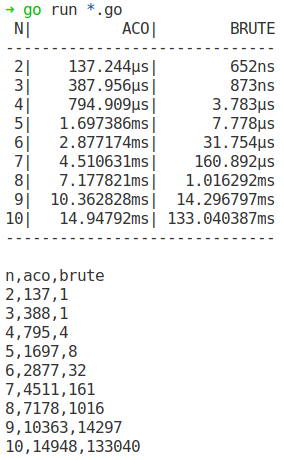
\includegraphics[width=0.4\textwidth]{6/inc/e1.png}
    \caption{Примеры работы программы}
    \label{fig:4.1}
\end{figure}

\begin{figure}[h]
    \centering
    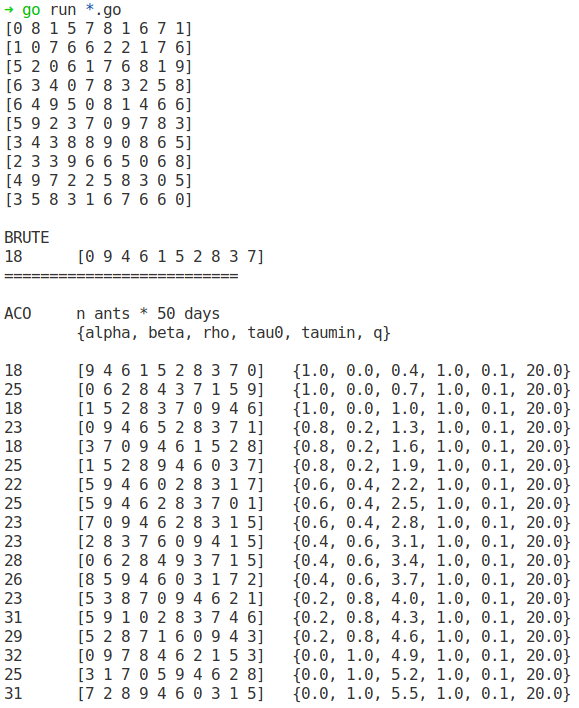
\includegraphics[width=0.8\textwidth]{6/inc/e2.png}
    \caption{Параметризация для матрицы размером 10 × 10}
    \label{fig:4.1}
\end{figure}



% \section{Постановка эксперимента по замеру времени}
\pagebreak
\section{Сравнение времени работы}

Операционная система - Ubuntu 20.04.1 LTS

Процессор - Intel® CoreTM i5-7300HQ CPU @ 2.50GHz × 4 (ЦП 4 ядра 4 потока)

В таблице \ref{tabular:benchmark} приведены замеры времени работы
реализации алгоритмов решения задачи коммивояжера.


% \def\arraystretch{1.2}
\setlength\tabcolsep{0.2cm}

\begin{table}[h]
    \centering
    \csvreader[tabular=|c|c|c|c|,
        table head=\hline
        \bfseries Размер
        & \bfseries Муравьиный
        & \bfseries Перебор
        \\\hline,
        late after line=\\\hline]
        {6/inc/benchmark.csv}{}
    { \csvcoli & \csvcolii & \csvcoliii}
    \caption{\label{tabular:benchmark} Время работы ($\mu$с)}
\end{table}


% \clearpage
\begin{figure}[!h]
    \centering
    \begin{tikzpicture}
        \begin{axis}[
            scale=1.6,
            axis lines=left,
            xlabel=Размер матрицы,
            ylabel={Время, $\mu$с},
            legend pos=north west,
            xmajorgrids=true,
            ymajorgrids=true,
            ymin=0,
        ]
            \addplot table[x=n,y=aco,col sep=comma] {6/inc/benchmark.csv};
            \addplot table[x=n,y=brute,col sep=comma] {6/inc/benchmark.csv};
            \legend{Муравьиный, Перебор}
        \end{axis}
    \end{tikzpicture}
    \caption{Зависимость времени работы реализации алгоритмов решения задачи коммивояжера от размерности}
    \label{fig:4.4}
\end{figure}

\pagebreak
\section{Вывод}

График показывает, что муравьиный алгоритм решения задачи коммивояжера выигрывает
у алгоритма полного перебора начиная с графа, количество вершин в котором больше 8.
Решение методом грубой силы становится непрактичным даже для 20 городов.
С плохими параметрами конфигурации муравьиный алгоритм может «застрять» на локальных экстремумах